\documentclass[a4paper,10pt]{article}
\usepackage[italian,english]{babel}
\usepackage[a4paper]{geometry}
\usepackage{amsmath}
\usepackage{amssymb}
\usepackage{bm}
\usepackage{graphicx}
\usepackage[authoryear]{natbib}
\usepackage{fancyvrb}
\usepackage{mathpazo}

\newcommand{\eps}{\varepsilon}
\newcommand{\Wb}{\mathbf{W}}
\newcommand{\wb}{\mathbf{w}}
\newcommand{\Xb}{\mathbf{X}}
\newcommand{\xb}{\mathbf{x}}
\newcommand{\Yb}{\mathbf{Y}}
\newcommand{\yb}{\mathbf{y}}
\newcommand{\Zb}{\mathbf{Z}}
\newcommand{\zb}{\mathbf{z}}
\newcommand{\zerob}{\boldsymbol{0}}
\newcommand{\bb}{\boldsymbol{\beta}}
\newcommand{\Sp}[1]{\mathrm{\left(#1\right)}}

\DefineVerbatimEnvironment%
{code}{Verbatim}
% original:
% {fontsize=\small, xleftmargin=1em}
{fontsize=\footnotesize, xleftmargin=1em}

% ----------------------------------------------------------------------

\newenvironment{funcdoc}[1]
{\noindent\hrulefill\newline\texttt{#1}\par\noindent\hrulefill\par\medskip\par}
{\bigskip}

% ----------------------------------------------------------------------
\newcommand{\gretl}{\textsf{gretl}}
\newcommand{\pder}[2]{\ensuremath{\frac{\partial #1}{\partial #2}}}

\author{Riccardo (Jack) Lucchetti \and Allin Cottrell}

\date{version 2.0}

\title{The \textsf{DynMultCalc} package}

\begin{document}

\maketitle

\begin{abstract}
  This gretl package provides an easy way to compute the dynamic
  multipliers from an autoregressive-distributed lag model. A
  graphical interface is also provided.
\end{abstract}

\section{Methods}

This package implements the calculation of dynamic multipliers for ADL
models, defined as
\begin{equation}
  \label{eq:ADL}
  y_t = \mu_t + \sum_{i=1}^p \alpha_i y_{t-i} + \sum_{i=0}^q
  \bb_i' \xb_{t-i} + \eps_t
\end{equation}
or, in lag notation, $A(L) y_t = \mu_t + B(L) \xb_t + \eps_t$.
Dynamic multipliers can be thought of as the parameters of the
rational polynomial
\begin{equation}
  \label{eq:DynMult}
  D(L) = \frac{B(L)}{A(L)} = \sum_{i=0}^{\infty} \delta_i L^i .
\end{equation}
Among other quantities of interest that one can calculate from the
multipliers $\delta_i$ are the ``cumulated'' (also known as
``interim'') multipliers $ c_k = \sum_{i=0}^k \delta_i$, the long-run
multiplier
\[
  c = \lim_{k \to \infty} c_k = \sum_{i=0}^{\infty} \delta_i = D(1)
\]
and the mean lag, which is defined only when the multipliers have all
the same sign, as
\[
  \lambda = \frac{\sum_{i=0}^{\infty} i \delta_i}{\sum_{i=0}^{\infty} \delta_i}.
\]
It can be proven that $\lambda$ can be written as
\[
  \lambda = \frac{B'(1)}{B(1)} - \frac{A'(1)}{A(1)}, 
\]
where the prime symbol indicates differentiation; this is the formula
used in the package.

Note that no estimation is carried out in the package. The parameters
in equation \eqref{eq:ADL} may be estimated or fixed by the user. In
the former case the estimation method is left to the user; it will
typically be OLS, but not necessarily (for example, the \texttt{ADMBP}
package by A. Tarassow implements several advanced techniques). In
fact, the \texttt{DynMultCalc} package will work as long as the user
supplies an input bundle containing the following keys:

\medskip
\begin{center}
\begin{tabular}{llp{0.63\textwidth}}
  \hline
  \textbf{Type} & \textbf{Key name} & \textbf{Content} \\
  \hline
  string & \texttt{depvar} & Name of the dependent variable $y_t$ \\ 
  list & \texttt{xlist} & List of independent variables
                          $\xb_t$ \\ 
  strings & \texttt{xnames} & String array with the names of $\xb_t$
                              and its lags \\ 
  matrix & \texttt{coeff} & $k \times 1$ vector with the model parameters   \\ 
  matrix & \texttt{vcv} & $k \times k$ covariance matrix (used for
                          computing confidence intervals) \\
  \hline
\end{tabular}
\end{center}

\medskip

In most cases the user will want to estimate a model using the ordinary
gretl estimation commands and then use the \verb|$model| accessor bundle.
Standard errors are computed via the delta method. This covers both
the stationary and cointegrated cases, under the provisos described in
\cite{PesaranShin1998}.

\section{Scripting usage}
\label{sec:scripting}

The package can be used in scripts as follows: after loading the
package, one sets up the model bundle and passes it to the
\texttt{multipliers} function, which returns a bundle with the
quantities of interest. The auxiliary functions \texttt{multi\_print}
and \texttt{multi\_plot} can be used to inspect its content. Here's an
example script:

\begin{code}
set verbose off
open denmark                   # open a dataset
include DynMultCalc.gfn        # include the package

# estimate a model (with minimal output)
ols LRM const LRM(-1 to -2) LRY(0 to -2) IBO(0 to -1) IDE(0 to -2) --simple

# compute the multipliers for LRY from the last estimated model
mb = multipliers($model, "LRY")

# print the multipliers
multi_print(mb)
\end{code}
%$
The script above gives the output shown below. Note that the
\texttt{multipliers} function simply takes the bundle containing the
model as its first argument, plus a string to identify the independent
variable for which the multipliers are wanted.

\begin{scriptsize}
\begin{code}
OLS, using observations 1974:3-1987:3 (T = 53)
Dependent variable: LRM

             coefficient   std. error   t-ratio   p-value 
  --------------------------------------------------------
  const        2.01750      0.481545     4.190    0.0001   ***
  LRM_1        0.249916     0.140445     1.779    0.0824   *
  LRM_2        0.444696     0.119450     3.723    0.0006   ***
  LRY          0.677771     0.139388     4.862    1.66e-05 ***
  LRY_1       -0.153798     0.194449    -0.7909   0.4334  
  LRY_2       -0.231809     0.156326    -1.483    0.1456  
  IBO         -1.11316      0.362915    -3.067    0.0038   ***
  IBO_1       -0.450343     0.483910    -0.9306   0.3574  
  IDE          0.664906     0.586319     1.134    0.2632  
  IDE_1       -0.308501     0.765299    -0.4031   0.6889  
  IDE_2        0.583660     0.517314     1.128    0.2656  

SSR = 0.0189294, R-squared = 0.984416

ADL(2, 2) model;
Multipliers of LRM to LRY


             coefficient   std. error     z     p-value 
  ------------------------------------------------------
  Long-run    0.956694      0.195604    4.891   1.00e-06 ***

Mean lag =  1.62 quarters

             coefficient   std. error      z      p-value 
  --------------------------------------------------------
  LRY_00     0.677771      0.139388     4.862     1.16e-06 ***
  LRY_01     0.0155873     0.176712     0.08821   0.9297  
  LRY_02     0.0734881     0.125389     0.5861    0.5578  
  LRY_03     0.0252974     0.0569678    0.4441    0.6570
  [...]
  LRY_17     0.00182019    0.00138633   1.313     0.1892  
  LRY_18     0.00146711    0.00117267   1.251     0.2109  
\end{code}
\end{scriptsize}

If you want to compute multipliers for an horizon different than the
default value (18), you can supply that as a third optional argument, as in
\begin{code}
  mb = multipliers($model, "LRY", 24)  
\end{code}
% $

\subsection{All long-run effects}
\label{sec:LR}

If you just want to examine the long-run effects of all the exogenous
variables on the dependent variable, the \texttt{long\_run\_effects}
function and its companion, \texttt{long\_run\_print}, should meet
your needs. Section~\ref{sec:functions} below contains a full
description of these functions, but a simple adaptation of the example
above should make their usage clear: the code below

\begin{code}
set verbose off
open denmark                   # open a dataset
include DynMultCalc.gfn        # include the package

# estimate a model (with minimal output)
ols LRM const LRM(-1 to -2) LRY(0 to -2) IBO(0 to -1) IDE(0 to -2) --quiet

# compute the long-run multipliers
bundle lr_fx = long_run_effects($model)

# print the long-run multipliers
long_run_print(lr_fx)
\end{code}
%$

\noindent produces the following output:

\begin{code}
Long-run effects on LRM, all exogenous regressors

             coefficient   std. error     z      p-value 
  -------------------------------------------------------
  LRY          0.956694     0.195604     4.891   1.00e-06 ***
  IBO         -5.11971      0.927033    -5.523   3.34e-08 ***
  IDE          3.07825      1.56915      1.962   0.0498   **

Mean lags (quarters):

LRY       1.6174 
IBO       4.0187 
IDE       4.6443 
\end{code}


\subsection{Special case: MA representation of $A(L)$}
\label{sec:MArep}

In some cases it may be interesting to compute multipliers with
respect to the disturbance term $\eps_t$ in Equation \eqref{eq:ADL},
that is, the response of the dependent variable to a unit random
shock. In this case, the polynomial $B(L)$ in Equation
\eqref{eq:DynMult} becomes $B(L) = 1$ and the multiplier sequence is
simply the MA representation of the autoregressive polynomial $A(L)$.

This can be obtained by using the name of the dependent variable as
the second argument to the \texttt{multipliers()} function, as in, for
example,
\begin{code}
ols LRM const LRM(-1 to -2) LRY(0 to -2) IBO(0 to -1) IDE(0 to -2) --simple
mb = multipliers($model, "LRM")
multi_print(mb)  
\end{code}
%$
\section{GUI usage}
\label{sec:GUI}

If you estimate a model in gretl's graphical interface via \emph{Model
  $>$ Ordinary Least Squares}, and the specification includes a lagged
dependent variable and/or one or more lagged independent variables,
then---assuming the \textsf{DynMultCalc} package has been correctly
installed---you will find a ``Dynamic Multipliers'' item at the foot
of the drop-down ``Analysis'' menu, as shown in the left-hand pane of
Figure~\ref{fig:sshot}.

\begin{figure}[hbtp]
  \caption{Example screenshots}
  \label{fig:sshot}
  \begin{center}
  \begin{tabular}{cc}
    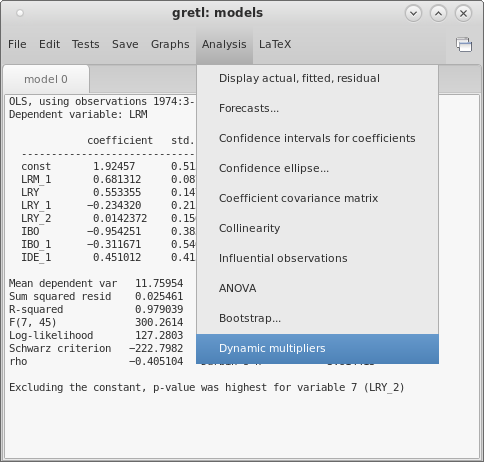
\includegraphics[width=6cm]{modelwin.png} &
    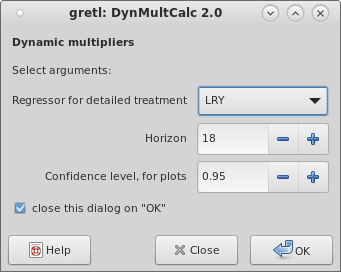
\includegraphics[width=6cm]{GUI_main.png}
  \end{tabular}
  \end{center}
\end{figure}

Clicking on this item opens a dialog box similar to that shown in the
right-hand panel of Figure~\ref{fig:sshot}. You can choose the
independent variable for which multipliers will be computed from the
drop-down list.\footnote{The ``MA representation'' option described in
  Section \ref{sec:MArep} is not available in this context.} The
outcome will be a window showing the long-run multipliers for all of
the independent variables followed by the output of the
\texttt{multi\_print} function.

Additionally, you will see some icons in the toolbar at the top of the output window, one of which
(the second from the right) calls for plotting. Click on it to get the choice of plotting the
sequence of dynamic or cumulated multipliers, with a confidence band drawn in accordance with the
argument given. Examples of such plots are shown in Figure \ref{fig:mults}. You can use the context
menu (right-click on most systems) to customize the plot to your liking and/or save it to a
\textsf{pdf} or \textsf{png} file.

\begin{figure}[htbp]
  \label{fig:mults}
  \begin{center}
  \begin{tabular}{c}
    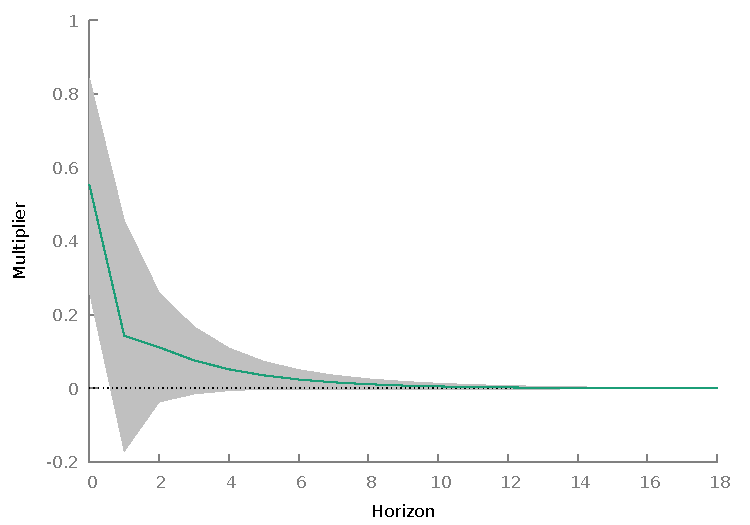
\includegraphics[scale=0.75]{m_example} \\[10pt]
    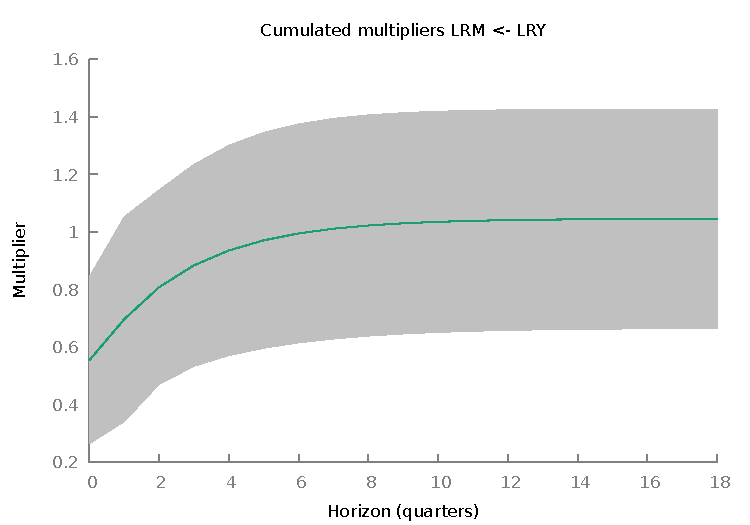
\includegraphics[scale=0.75]{cm_example}
  \end{tabular}
  \caption{Plots available via the \textsf{DynMultCal} graphical
    interface}
  \end{center}
\end{figure}
\clearpage
\section{Alphabetical list of public functions}
 \label{sec:functions}


\begin{funcdoc}{long\_run\_effects(bundle model)}
  \begin{description}
  \item[Return type]: \texttt{bundle}
  \item[\texttt{model}]: a model bundle, typically obtained via the
    \verb|$model| accessor after estimation.
\end{description}
%

\noindent Computes the long-run multipliers for a dynamic model. The
output of the function is a bundle containing the following keys:

\medskip
\begin{center}
\begin{tabular}{llp{0.63\textwidth}}
  \hline
  \textbf{Type} & \textbf{Key name} & \textbf{Content} \\
  \hline
  scalar & \texttt{LRMs} & a 2-column matrix holding the long-run multipliers
                           and their asymptotic standard errors \\ 
  matrix & \texttt{meanlags} & a matrix holding the mean lags where available \\ 
  string & \texttt{pdstr} & name of the time unit \\ 
  string & \texttt{yname} & name of the explanatory variable \\ 
  \hline
\end{tabular}
\end{center}
\end{funcdoc}

\begin{funcdoc}{long\_run\_print (bundle blr)}
  \begin{description}
  \item[Return type]: none
  \item[\texttt{blr}]: a bundle like the one produced by the
    \texttt{long\_run\_effects()} function.
\end{description}

\noindent Pretty-prints the long run multipliers.
\end{funcdoc}

\begin{funcdoc}{multipliers(bundle mod, string xname, int horizon)}
  \begin{description}
  \item[Return type]: \texttt{bundle}
  \item[\texttt{mod}]: the model bundle
  \item[\texttt{xname}]: the name of the variable you want the
    multipliers for (as a string)
  \item[\texttt{horizon}]: number of steps (default = 18)
\end{description}
%

\noindent The output of the function is a bundle containing the
following keys:

\medskip
\begin{center}
\begin{tabular}{llp{0.63\textwidth}}
  \hline
  \textbf{Type} & \textbf{Key name} & \textbf{Content} \\
  \hline
  scalar & \texttt{meanlag} & the mean lag \\
  matrix & \texttt{dyn\_mult} & a 2-column matrix holding the multipliers
                           and their asymptotic standard errors \\ 
  matrix & \texttt{cum\_mult} & a 2-column matrix holding the interim multipliers
                           and their asymptotic standard errors \\ 
  scalars & \texttt{p, q} & orders of the $A(L)$ and $B(L)$ polynomials \\
  scalar & \texttt{sdx} & standard deviation of the selected
                          independent variable \\
  matrix & \texttt{LRM} & a 2-vector holding the long-run multiplier
                          $c$ and its asymptotic standard error \\ 
  matrix & \texttt{xlags} & matrix holding the powers of the non-zero
                            elements of $B(L)$ \\ 
  matrix & \texttt{ylags} & matrix holding the powers of the non-zero
                            elements of $A(L)$ \\ 
  string & \texttt{xname} & name of the dependent variable \\ 
  string & \texttt{yname} & name of the explanatory variable \\ 
  \hline
\end{tabular}

\end{center}
Note: if \texttt{xname} is the name of the dependent variable of
the model, the multipliers will be the MA representation of the
autoregressive part of the model (see Section \ref{sec:MArep}). 
\end{funcdoc}


\begin{funcdoc}{multi\_plot(const bundle b, bool cumulate, scalar conflev,
			 string ofile)}
  \begin{description}
  \item[Return type]: \texttt{none}
  \item[\texttt{b}]: a bundle generated by the \texttt{multipliers} function.
  \item[\texttt{cumulate}]: boolean flag: 0 (the default) to plot the
    ordinary multipliers, $\delta_i$, or 1 to plot the cumulated
    (``interim'') ones $c_i$
  \item[\texttt{conflev}]: a scalar between 0 and 1, with the
    confidence level for the plotted band; if omitted, it defaults at 0.95.
  \item[\texttt{ofile}]: an optional string for redirecting the output.
\end{description}
\noindent Plots the multiplier with a confidence band. If the
\texttt{ofile} parameter is omitted the plot will be produced on
screen. Otherwise, the plot will be saved under the specified name,
with format determined by the file's extension, such as \texttt{.pdf}
or \texttt{.png}. Note that it's the user's responsibility to give a
valid filename.  
\end{funcdoc}

\begin{funcdoc}{multi\_print(const bundle b)}
  \begin{description}
  \item[Return type]: \texttt{none}
  \item[\texttt{b}]: a bundle generated by the \texttt{multipliers} function.
\end{description}
\noindent Prints out the quantities of interest.
\end{funcdoc}


%\clearpage
\bibliographystyle{jae}
\bibliography{DynMultCalc}

\section*{Changelog}
\addcontentsline{toc}{section}{Changelog}
\begin{itemize}
\item \texttt{v2.0}: GUI hook by Allin and various other internal
  refinements. Add the ``MA representation'' facility and the two
  ``long run'' functions.
\item \texttt{v1.0}: Initial release.
\end{itemize}

\end{document}

%%% Local Variables:
%%% mode: latex
%%% TeX-master: t
%%% End:
